\documentclass{article} % For LaTeX2e
\usepackage{nips14submit_e,times}
\usepackage{hyperref}
\hypersetup{pdfstartview={FitH},colorlinks=false,pdfborder={0 0 0},}
\usepackage{url}
\usepackage{amsmath}
\usepackage{graphicx}
\usepackage{hhline}
\newcommand{\lr}{\text{learningRate}}
\newcommand{\cost}{\text{cost}}
\newcommand{\mask}{\text{mask}}
%\documentstyle[nips14submit_09,times,art10]{article} % For LaTeX 2.09


\title{Deep Learning With Noise}

\author{
Yixin Luo \\
Computer Science Department \\
Carnegie Mellon University \\
\texttt{yixinluo@cs.cmu.edu} \\
\And
Fan Yang\\
Department of Mathematical Sciences \\
Carnegie Mellon University \\
\texttt{fanyang1@andrew.cmu.edu} \\
}

% The \author macro works with any number of authors. There are two commands
% used to separate the names and addresses of multiple authors: \And and \AND.
%
% Using \And between authors leaves it to \LaTeX{} to determine where to break
% the lines. Using \AND forces a linebreak at that point. So, if \LaTeX{}
% puts 3 of 4 authors names on the first line, and the last on the second
% line, try using \AND instead of \And before the third author name.

\newcommand{\fix}{\marginpar{FIX}}
\newcommand{\new}{\marginpar{NEW}}

\nipsfinalcopy % Uncomment for camera-ready version

\begin{document}

\maketitle

% sections
\section{Introduction}
\label{sec:intro}

Large-scale deep neutral network models have become increasingly popular to
solve hard classification problems and have demonstrated significant
improvements in accuracy. Compared to traditional statistical machine learning
methods, which require a human domain expert that can construct a good set of
features as input dataset, deep learning models do not require a hand crafted
feature set to begin with, and hence is more powerful and suitable for hard AI
tasks such as speech recognition or visual object classification. Without any
hand crafting of the raw input data, deep neural network machine learning models
can learn a hierarchy of features by itself in the first several layers of
neural network model. Then, in the deepest layer of the model, a set of features
are selected and weighted for each output to generate a prediction. Avoiding the
inevitable human error in feature selection, deep learning often outperforms
traditional approaches in those hard classification problems in terms of
accuracy.

In order to train a more complicated model which includes feature selection
capability, deep neural network is typically trained with more data than a
traditional machine learning method. Due to the scale of the deep neutral
network (with multiple layers of neurons) and the scale of the input data set,
the performance of these models, in addition to accuracy, has become a
significant factor in such implementations. Recent
work~\cite{chilimbi14adam,wan2013dropconnect} on large-scale machine learning
systems propose to significantly improve the performance by relaxing the
consistency when training neural network models (e.g.,  weights will not be
updated in each iteration). One interesting observation in these papers,
alongside the above one, is that relaxation surprisingly improves the {\em
accuracy} of the deep learning model on the test data.

However, the effect of noise on deep learning models has never been
systematically studied, nor is the underlying reason for the improved accuracy.
One hypothesis of the above observation is that relaxing consistency introduces
stochastic noise into training process~\cite{chilimbi14adam}.  This implicitly
mitigates over-fitting of the model and generalizes the model better to classify
test data. Another hypothesis of this observation is that the introduced noise
eliminates the memorization effect of a deep neural network, and hence allows
the model to capture the general observation of the training data that can be
applied to the test data well.

Our work, taking previous works as examples and guidance, tries to
study the effect of introducing different noise into different
components of deep learning neural networks. We focus on introducing
noise into training process of neural networks instead of into dataset.
We hope that our work can provide insights into future exploration of
hardware approximate computation/storage techniques to accelerate and
improve the accuracy of large-scale deep learning models.

% Related works?

\section{Background and Related Work}
\label{sec:problem}

In this section, we first introduce several common neural networks model,
Logistic Regression (single neuron) model, Multi-Layer Perceptron (MLP) model,
and Convolutional Neural Network (LeNet) model. Then we summarize and compare
our work to several related works that introduce noise into those models to
improve accuracy.

\subsection{Neural Network Models Explained}

The simplest form of a neural network, which is also the primary component of
any neural network model, is a single neuron. Figure~\ref{fig:lr-diag} illustrates a
single-neuron neural network, which is also known as the Logistic Regression
(LR) model. The neuron shown in the figure consumes a vector of numbers (X) as
inputs, and produces a single number as its output, which typically represents
the prediction result by the model. The neuron stores a vector of weights (W),
with each weight represents how positively or negatively each input affects the
output. The output of the neuron and the update to the neuron's weight can be
computed as follows:
\[
  Output = \tanh(W \cdot X)
\]
\[
  W_{new} = W_{old} - learningRate \cdot \nabla_{W_{old}} \cost(W)
\]

A Multi-Layer Perceptron (MLP) model is essentially multiple layers of neurons
connected by a network. Figure~\ref{fig:mlp-diag} illustrates a simple example of
such model, which is composed of three layers. The first layer is the input
layer, which provides the raw inputs to the next layer. The second layer is the
hidden layer, whose input is fully connected to the input layer, and output
fully connected to the output layer. The hidden layer is known to be capable of
extracting features from the input. The third layer is the output layer, which
outputs the prediction results for the data. Note that the figure shows only an
example of such model, the model can become ``deeper'' to extract more implicit
features from the raw input if we add more hidden layers between input and
output layers, which are fully connected to the layers next to each other.

\begin{figure}[!h]
\centering
\begin{subfigure}{.49\linewidth}
  \centering
  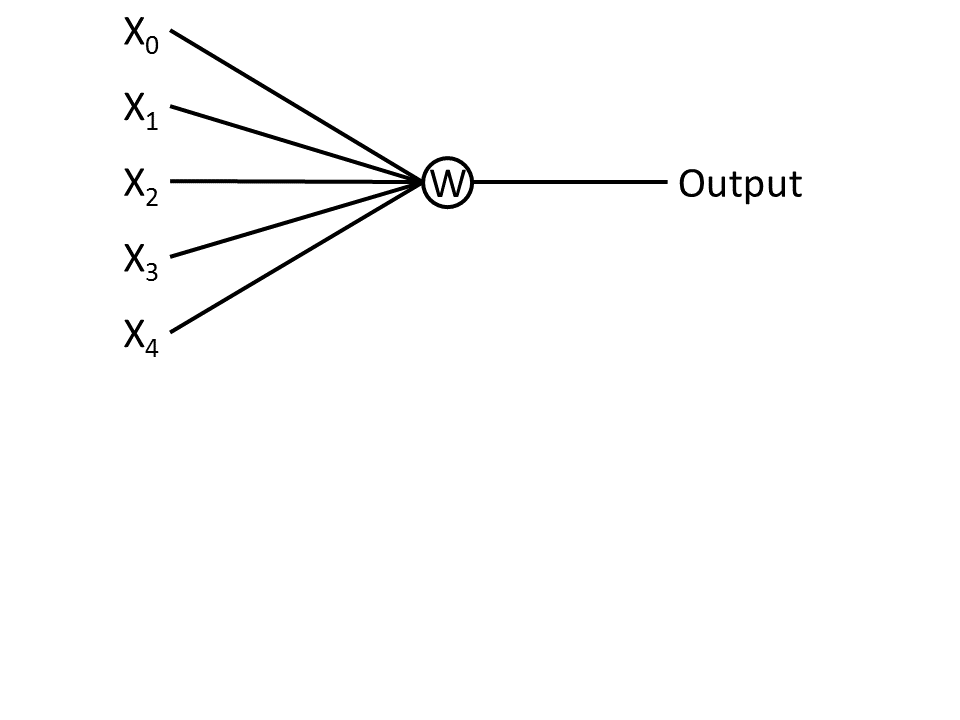
\includegraphics[trim=0 260 0 0,clip,width=\linewidth]{f-figs/lr-diag}
  \caption{Single-layer neural network (LR) model.}
  \label{fig:lr-diag}
\end{subfigure}
\begin{subfigure}{.5\linewidth}
  \centering
  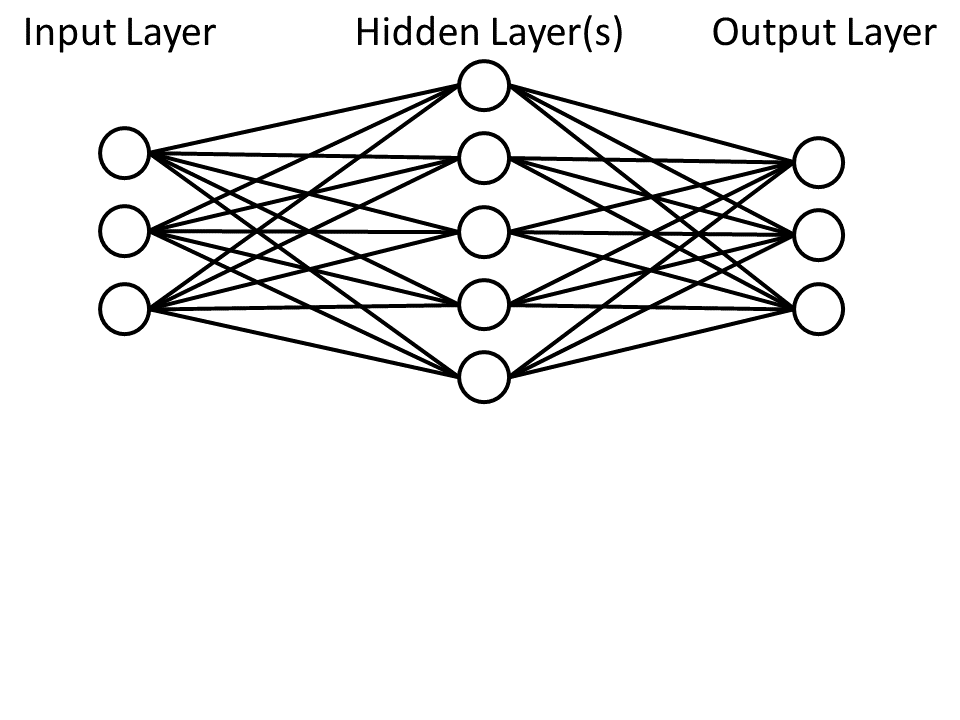
\includegraphics[trim=0 230 0 0,clip,width=\linewidth]{f-figs/mlp-diag}
  \caption{Multi-Layer Perceptron (MLP) model.}
  \label{fig:mlp-diag}
\end{subfigure}
\caption{Illustration of two neural network models.}
\end{figure}

A Convolutional Neural Network (LeNet) model adds multiple convolution layers in
addition to the MLP model. Figure~\ref{fig:lenet-diag} illustrates an example of this
model. In the convolution layer, multiple steps are processed. First, the input
is transformed into a two-dimensional array. Then a sliding window which
contains a small two-dimensional weight vector is applied to the input. The
sliding window is capable of extracting 2-D features from the inputs such as
images. Finally, the processed input is downsampled by a 2x2 matrix, which
reduces the size of the input by 4. In this figure, we show an example which
contains two convolution layer and a hidden layer. We can also have a more
complex model by adding more convolution layers or more hidden layers, which
also allows the model to extract more implicit features.

\begin{figure}[!h]
\centering
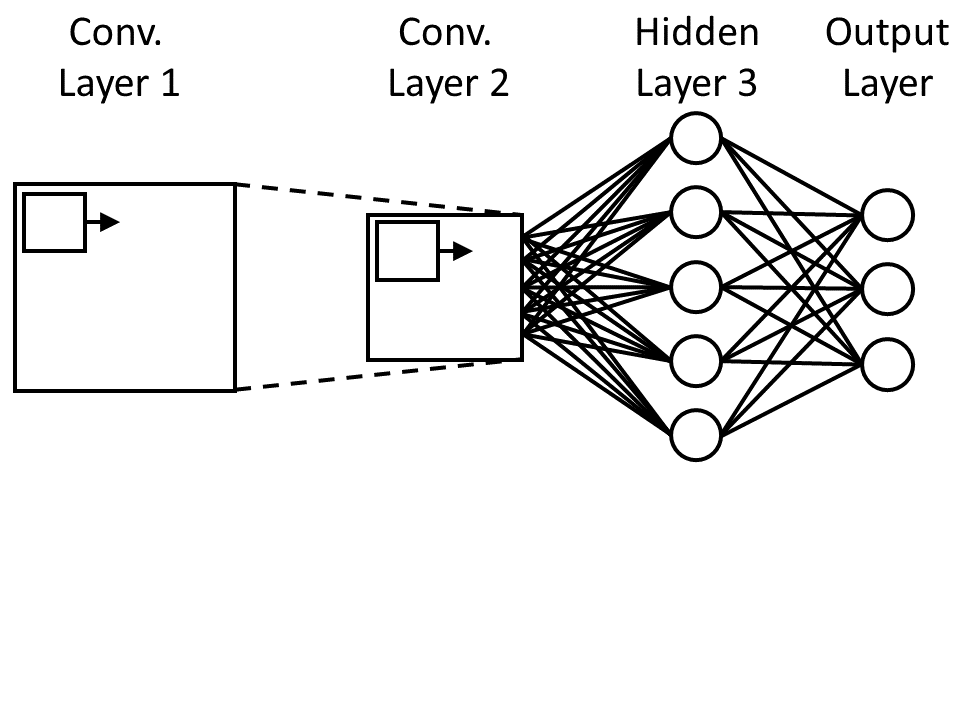
\includegraphics[trim=0 190 0 0,clip,width=0.6\linewidth]{f-figs/lenet-diag}
\caption{Convolutional Neural Network (LeNet) model.}
\label{fig:lenet-diag}
\end{figure}

\subsection{Comparison with Related Works}

We summarize three recent works that explain and explore three mechanisms to
introduce noise into a multi-layer neural network (mlp). Dropout proposes to
regularize fully connected neural networks by probabilistically dropping an
output (set to zero) of a hidden layer neuron~\cite{hinton2012improving} (i.e.,
with a low probability $(1-p)$, one of the output of a hidden layer neutron is
set to $0$ in the forward propagation process).  This can effectively decrease
test error rates by preventing over-fitting of the model. Inspired by
Dropout~\cite{hinton2012improving}, DropConnect proposes to probabilistically
drop a weight of a hidden layer neuron (as opposed to an output of a hidden
layer neuron in DropConnect)~\cite{wan2013dropconnect}. Maxout extends Dropout
and DropConnect by probabilistically set an output or a weight of a hidden layer
neuron to maximum value~\cite{goodfellow13maxout}. While these works attempts to
explore similar ideas as our work, we believe our work is much more
comprehensive than these works as we systematically and experimentally explored
various noise models, various noise locations, and various neural networks.




\section{Methodology}
\label{sec:meth}

%Data set (5 points): Is the data set completely ready (in-hand, loaded onto a machine, analyzed for outliers or other problems)? Have some main features of the data set been characterized (either visually or statistically)?


\subsection{MNIST}
MNIST is a data set of handwritten digits. It contains a training set of
60,000 examples and a test set of 10,000 examples. The digits have been
size-normalized and centered in a fixed-size image.

We used this data set in our first step experiments. (See Experiments for
more details.)

\subsection{CIFAR-10}
CIFAR-10 is a data set of 60000 32x32 colour images in 10 classes, with
6000 images per class. There are 50000 training images and 10000 test
images. The dataset is divided into five training batches and one test
batch, each with 10000 images. The test batch contains exactly 1000
randomly-selected images from each class. The training batches contain the
remaining images in random order, but some training batches may contain
more images from one class than another. Between them, the training
batches contain exactly 5000 images from each class.

We have succesfully loaded this dataset, and we are working on
fine-tuning parameters of the model to better fit this dataset.

\subsection{Other data sets}
Besides the above two datasets, we will conduct experiements on the
following datasets as well:
\begin{itemize}
\item CIFAR-100 \\
\item Street View House Numbers(SVHN)\\
\item
\end{itemize}


\section{Experiments}
\label{sec:experiments}

% Description of your testbed;
% List of questions your experiments are designed to answer.
% Details of the experiments; observations.
\subsection{Dataset and Implementation Parameters}
We experiment on three datasets---a hand-written digit dataset (MNIST),
two tiny images datasets (CIFAR-10 and CIFAR-100).
Specifications of datasets are summarized in Table~\ref{datasets}.
\vspace{-7pt}
\begin{table}[!htbp]
\centering
\begin{tabular}{| c | c | c | c | c |}
\hline
Dataset & Description & Class & Training Set Size & Testing Set Size \\
\hline
MNIST & hand-written digists & 10 & 60,000 & 10,000\\
CIFAR-10 & 32x32 RGB images & 10 & 50,000 & 10,000\\
CIFAR-100 & 32x32 RGB images & 10 & 50,000 & 10,000\\
\hline
\end{tabular}
\caption{Datasets: MNIST, CIFAR-10, CIFAR-100}
\label{datasets}
\end{table}

We preprocess CIFAR-10 and CIFAR-100 by grey-scaling every image using the following formula:
\[
Y = 0.2126 * R + 0.7152 * G + 0.0722 * B
\]
In other words, every pixel in the image is now a linear combination of its
original RGB values. These two datasets are preprocessed due to technical
implementation limitations (which will be fixed after the deadline), not
machine learning theory reasons.

Our neural netwoek models are implemented using Python Theono Library. The
starter code is from DeepLearning.net. Parameters of each neural
network models are summarized in Table~\ref{params}.
\vspace{-7pt}
\begin{table}[!htbp]
\centering
\begin{tabular}{| c | c |}
\hline
Model & Parameters \\
\hline
Logistic Regression (LR) & learning rate = 0.13 \\
Multi-layer Logistic Regression (MLP) & LR + hidden units = 500 \\
Convolutional Neural Network & MLP + window size = 5x5, downsample = 2x2\\
\hline
\end{tabular}
\caption{Parameters of Neural Network Models}
\label{params}
\end{table}

We use stochastic logistic regression with learning rate = 0.13.
In Multi-layer Logistic Regression, there are 500 neurons in the hidden
layer. During feature mapping of Convolutional Neural Network, windows
are of size 5 by 5 and downsample is of size 2 by 2.

\subsection{Adding Noise into Logistic Regression}
Figure~\ref{logistic} shows test error rate using noise-free and
noise-added Logistic Regression on MNIST.
\begin{figure}[!htbp]
\centering
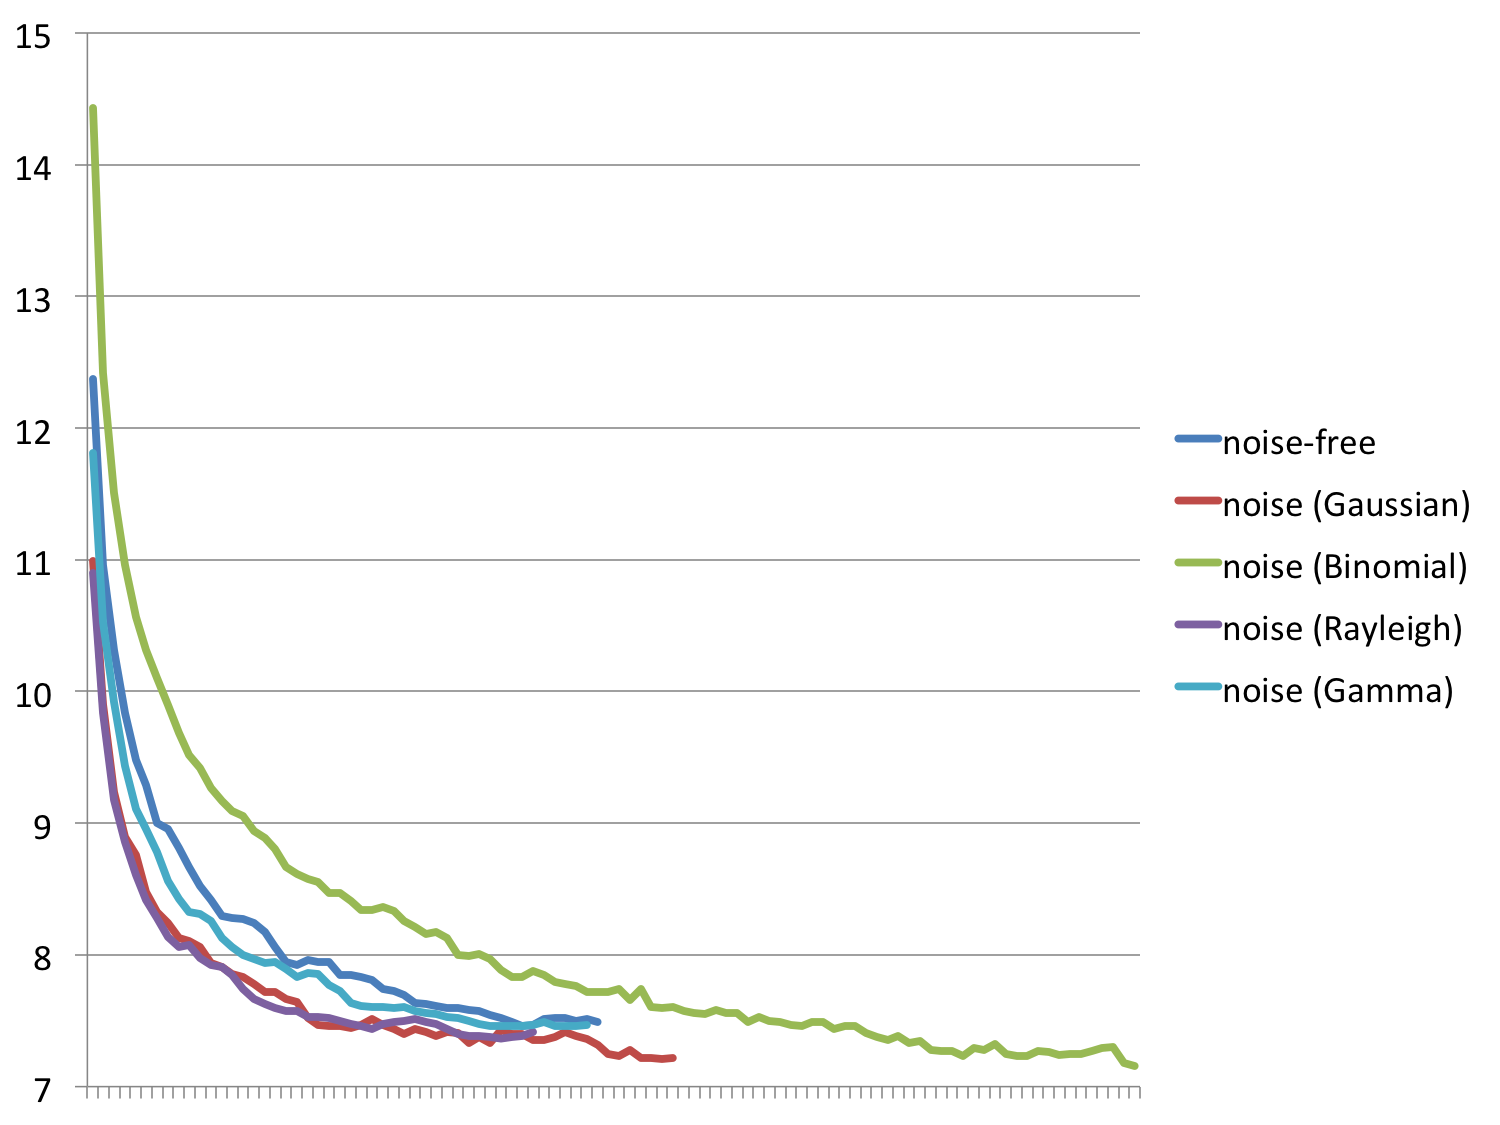
\includegraphics[width=295pt]{f-figs/logistic.png}
\caption{Logistic Regression with Noise on MNIST}
\label{logistic}
\end{figure}

% explain the figure

\subsection{Adding Noise into Multi-layer Logistic Regression}
Figure~\ref{mlp} shows test error rate using noise-free and noise-added
Multi-layer Logistic Regression on MNIST.
\begin{figure}[!htbp]
\centering
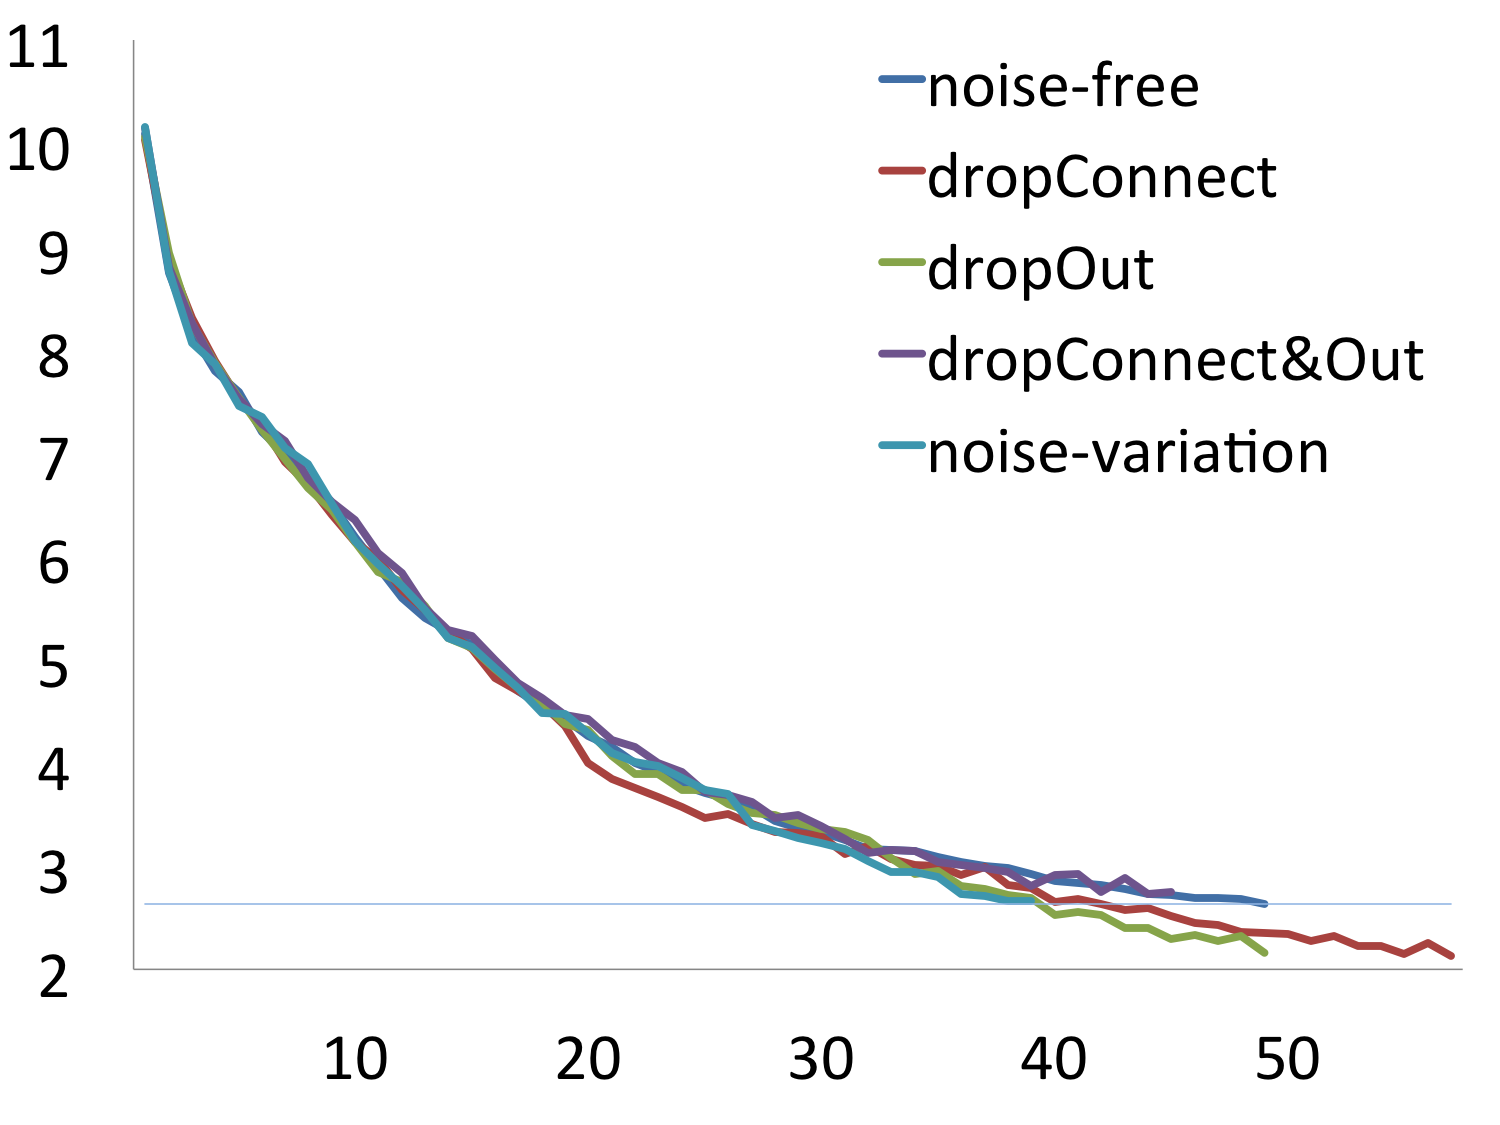
\includegraphics[width=295pt]{f-figs/mlp.png}
\caption{Multi-layer Logistic Regression with Noise on MNIST}
\label{mlp}
\end{figure}
% explain the figure

Figure~\ref{mlp10} shows test error rate using noise-free and noise-added
Multi-layer Logistic Regression on CIFAR-10.
\begin{figure}[!htbp]
\centering
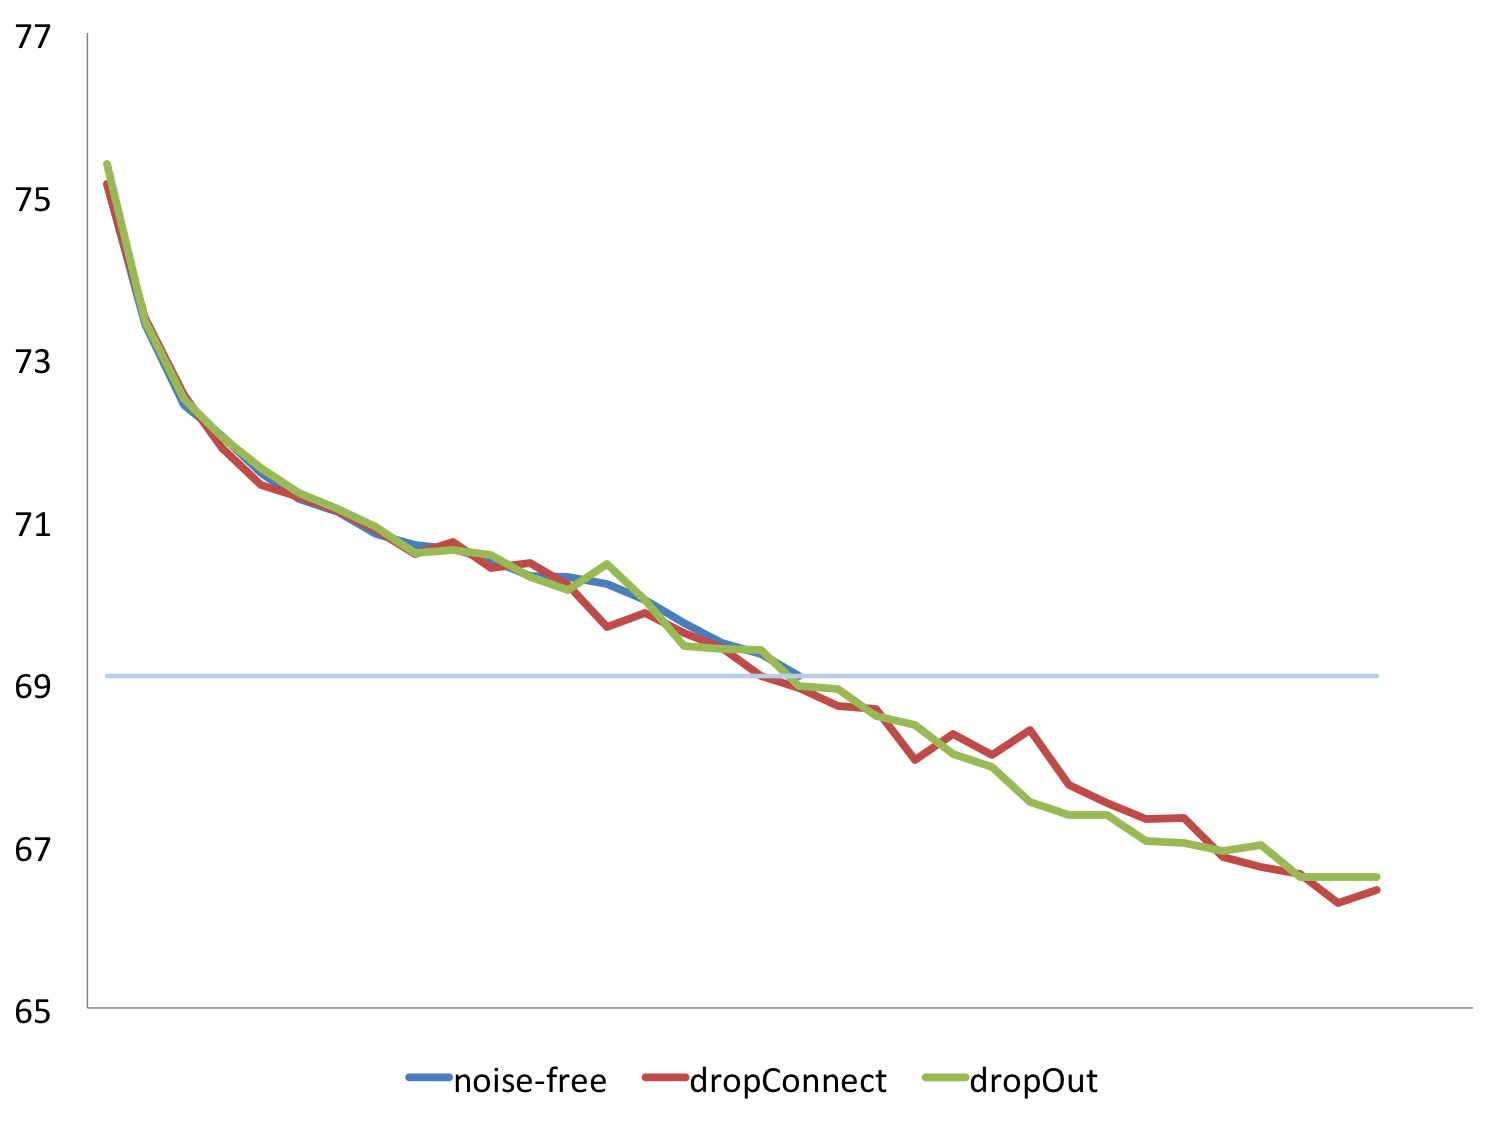
\includegraphics[width=295pt]{f-figs/mlp10.png}
\caption{Multi-layer Logistic Regression with Noise on CIFAR-10}
\label{mlp10}
\end{figure}
% explain the figure

\subsection{Adding Noise into Convolutionary Neural Network}
Figure~\ref{convo} shows test error rate using noise-free and noise-added
Convolutional Multi-layer Logistic Regression on MNIST.
\begin{figure}[!htbp]
\centering
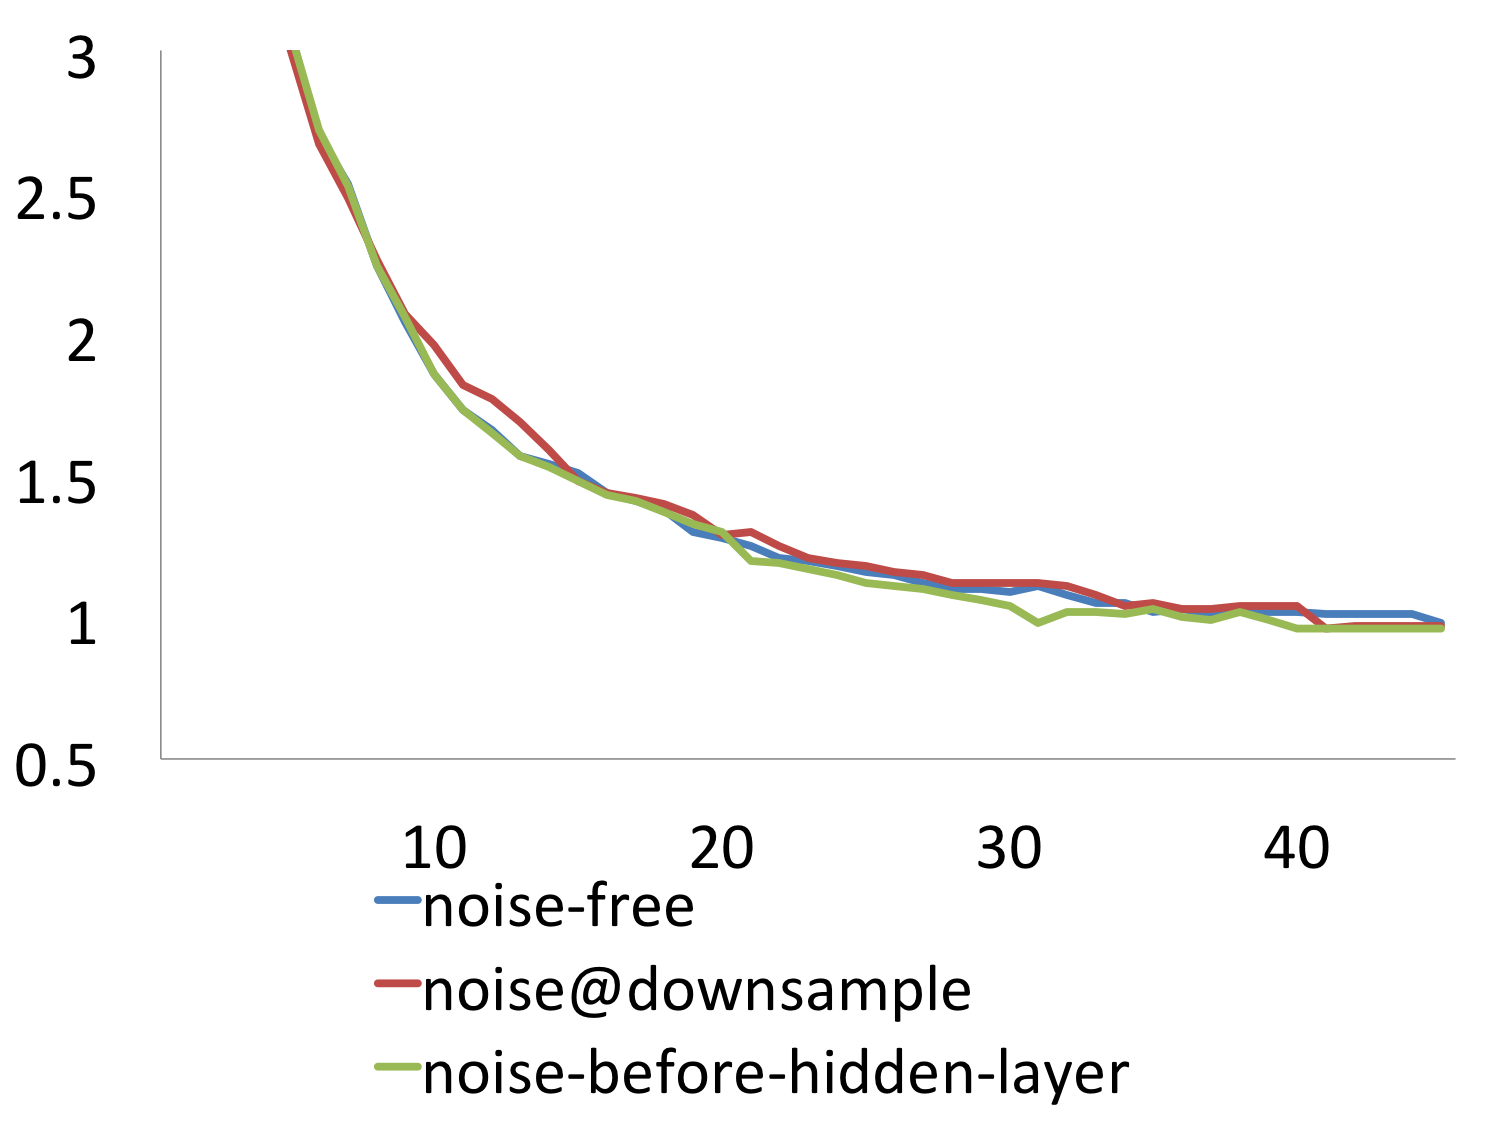
\includegraphics[width=295pt]{f-figs/convo.png}
\caption{Convolutionary Neural Network with Noise on MNIST}
\label{convo}
\end{figure}
% explain the figures

Figure~\ref{convo10} shows test error rate using noise-free and noise-added
Convolutional Multi-layer Logistic Regression on CIFAR-10.
\begin{figure}[!htbp]
\centering
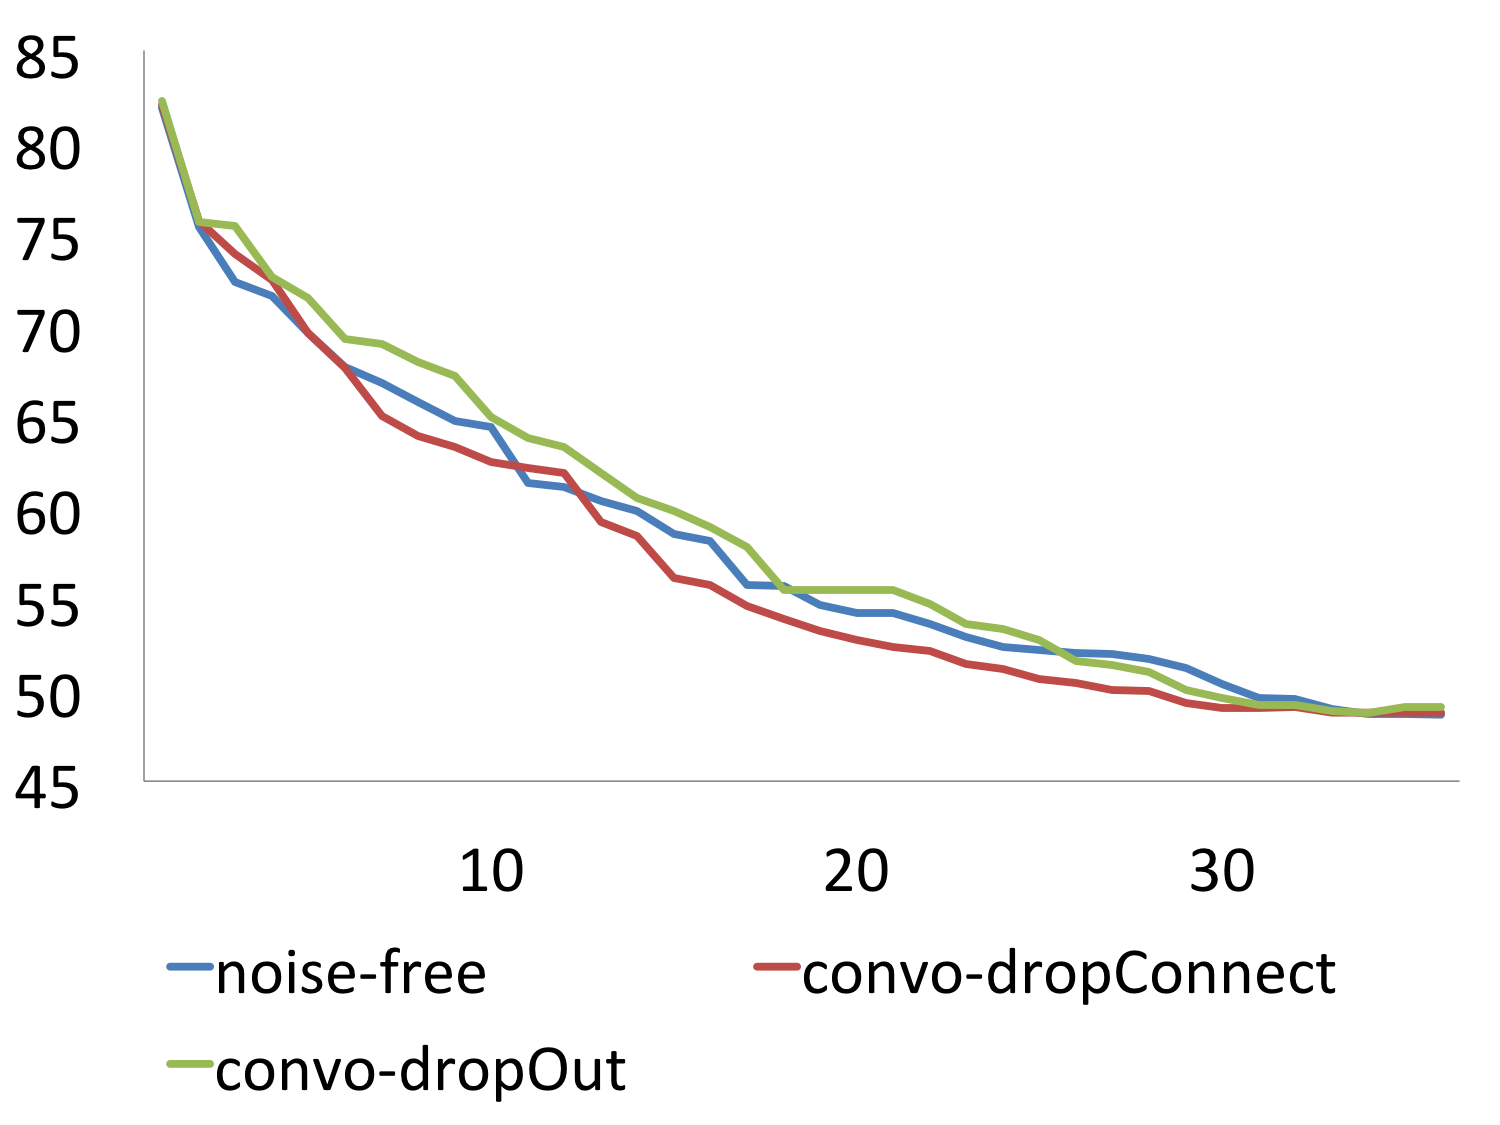
\includegraphics[width=295pt]{f-figs/convo10.png}
\caption{Convolutionary Neural Network with Noise on CIFAR-10}
\label{convo10}
\end{figure}

\section{Conclusions}
\label{sec:conclusions}
In this project, we systematically perform experiments on studying the
effect of adding noise into deep learning neural networks.
We conduct experiments on adding different noise into different components
of neural network models. The experiment results show that adding noise almost always improves accuracy.
Our main observations are:
(1) Noise added during early stage of the model can be better integrated
while noise added during late stage of the model tends to cause
fluctuation of accuracy;
(2) Complicated neural network models can integrate and absorb
noise better than simple neural network models;
(3) Sometimes adding noise can improve not only accuracy but also
convergence rate.
We hope that our experiment results can provide insight into future design
of deep learning neural network models and machine learning hardwares.

Beyond this project


\bibliographystyle{IEEEtran}
\bibliography{IEEEabrv,refs}

\end{document}
